\documentclass[12pt]{article}

\usepackage[margin=1in]{geometry}
\usepackage{amsfonts,amssymb,amsthm,amsmath,graphicx}
\usepackage{float}
\usepackage{listings}
\usepackage{hyperref}
\usepackage{verbatim}
\usepackage{mathtools}
\usepackage{enumitem}
\usepackage{xcolor}

\hypersetup{
    colorlinks,
    linkcolor={red!50!black},
    citecolor={blue!50!black},
    urlcolor={blue!80!black}
}

\definecolor{boxbackground}{rgb}{1,0.976, 0.882}

\lstset{
    language=Python,
    basicstyle=\scriptsize\ttfamily,
    keywordstyle=\color{blue}\ttfamily,
    stringstyle=\color{red}\ttfamily,
    commentstyle=\color{green!50!black}\ttfamily,
    frame=single,
    breaklines=true,
    postbreak=\raisebox{0ex}[0ex][0ex]{\ensuremath{\color{violet}\hookrightarrow\space}},
    backgroundcolor = \color{boxbackground},
    showspaces=false,
    showstringspaces=false,
}

\newcommand{\N}{\mathbb{N}}
\newcommand{\Z}{\mathbb{Z}}
\newcommand{\R}{\mathbb{R}}
\newcommand{\Q}{\mathbb{Q}}
\newcommand{\e}{\epsilon}
\newcommand{\C}{\mathbb{C}}
\newcommand{\norm}[1]{\left\lVert#1\right\rVert}
\newcommand{\li}[1]{\lstinline[prebreak=]!#1!}

\begin{document}
\title{Plotting with Pandas}
\author{Nathaniel Merrill, Shane McQuarrie, Amelia Henriksen, Marissa Graham}
\maketitle

\noindent \textbf{Objective:}
\emph{Pandas has many built-in plotting methods that wrap around matplotlib. Since Pandas provides tools for organizing and correlating large sets of data, it is important to be able to visualize these relationships. This lab consists of two parts: learning to plot with Pandas, and using those techniques to visualize data in informative ways.}
\\
\\
\noindent \textbf{Solutions Format:} \emph{IPython / Jupyter Notebook}

\section*{Plotting Data Frames}

% SHANE =======================================================================

Recall that in Pandas, a \emph{DataFrame} is an ordered collection of \emph{Series}.
A series is similar to a dictionary, with values assigned to various labels, or indices. Each series becomes a column in the data frame, with each row corresponding to an index.
When several series are combined into a single data frame, it becomes very easy to compare and visualize data.

%Every series is a column in the data frame, each sharing the same index.
%With several series in a single data frame, it very easy to compare and visualize data.

Data frames have several methods for easy plotting.
Most are simple wrappers around matplotlib commands, but some produce styles of plots that we have not previously seen.

% Using a Pandas dataframe to draw some familiar plots.
% Comparison between matplotlib and pandas code (show equivalent code and how pandas is easier).

% Do comparisons along the way of when one plot would be better than another.
% Be careful NOT to give the same examples as in the pandas documentation.

% Compare carefully the syntax with df.plot() vs. df.hist() and so on.
% Show how to make subplots and explain when it would or would not be helpful.

% Should we try to do everything with plot(), sometimes with plot(), or avoid plot() altogether?

% Compare pandas plots to Excel plots and convince people to use pandas instead of Excel.

For these examples, we will use the data found in the file \li{crime\_data.txt}.

\begin{lstlisting}
>>> import pandas as pd
>>> crime = pd.read_csv("crime_data.txt", header=1, index_col=0)
\end{lstlisting}

\subsection*{Line Plots}

Using matplotlib, we can plot the data in a single pandas \li{Series} against the data frame index (the years, in this case).
With a few extra lines we modify the $x$-axis label and limits and create a legend.

\begin{lstlisting}
>>> plt.plot(crime["Population"], label="Population")
>>> plt.xlabel("Year")
>>> plt.xlim(min(crime.index), max(crime.index))
>>> plt.legend(loc="best")
>>> plt.show()
\end{lstlisting}

Equivalently, we can produce the exact same plot with a single line using the DataFrame method \li{plot()}.
Specify the $y$ values as a keyword argument.
The $x$ values default to the index of the Series.
See Figure \ref{fig:intro}.

\begin{lstlisting}
>>> crime.plot(y="Population")
>>> plt.show()
\end{lstlisting}


\begin{figure}[H] % Matplotlib vs. Pandas 1
    \centering
    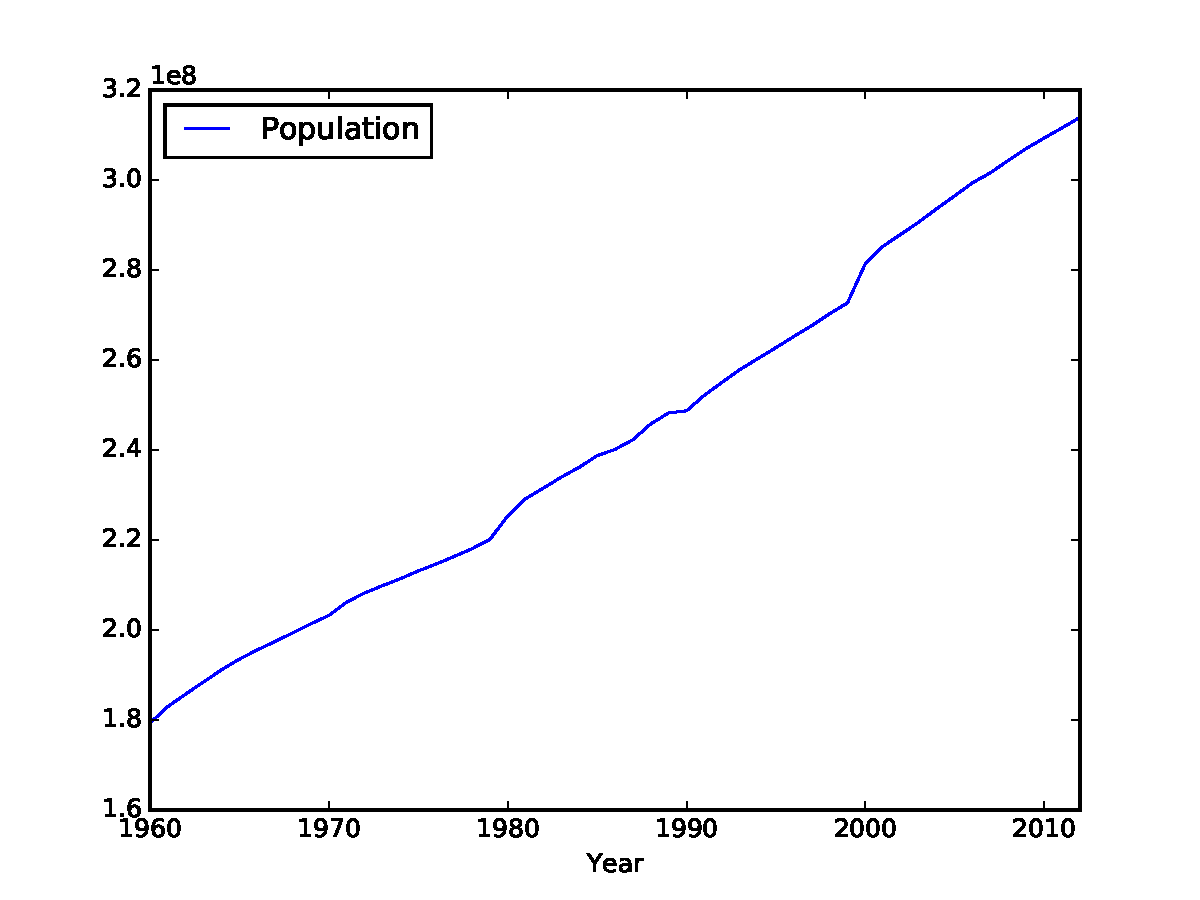
\includegraphics[scale=.5]{population.pdf}
    \caption{Population by Year.}
    \label{fig:intro}
\end{figure}

We can also plot two series against each other (ignoring the index).
In matplotlib:

\begin{lstlisting}
>>> plt.plot(crime["Population"], crime["Burglary"])
>>> plt.show()
\end{lstlisting}

With \li{DataFrame.plot()}, specify the $x$ values as a keyword argument:

\begin{lstlisting}
>>> crime.plot(x="Population", y="Burglary")
>>> plt.show()
\end{lstlisting}

Both procedures produce the same line plot, but the data frame method automatically sets the limits and labels of each axis and includes a legend.
See Figure \ref{fig:intro2}.

\begin{figure}[H] % Matplotlib vs. Pandas
    \centering
    \begin{minipage}[b]{0.48\textwidth}
    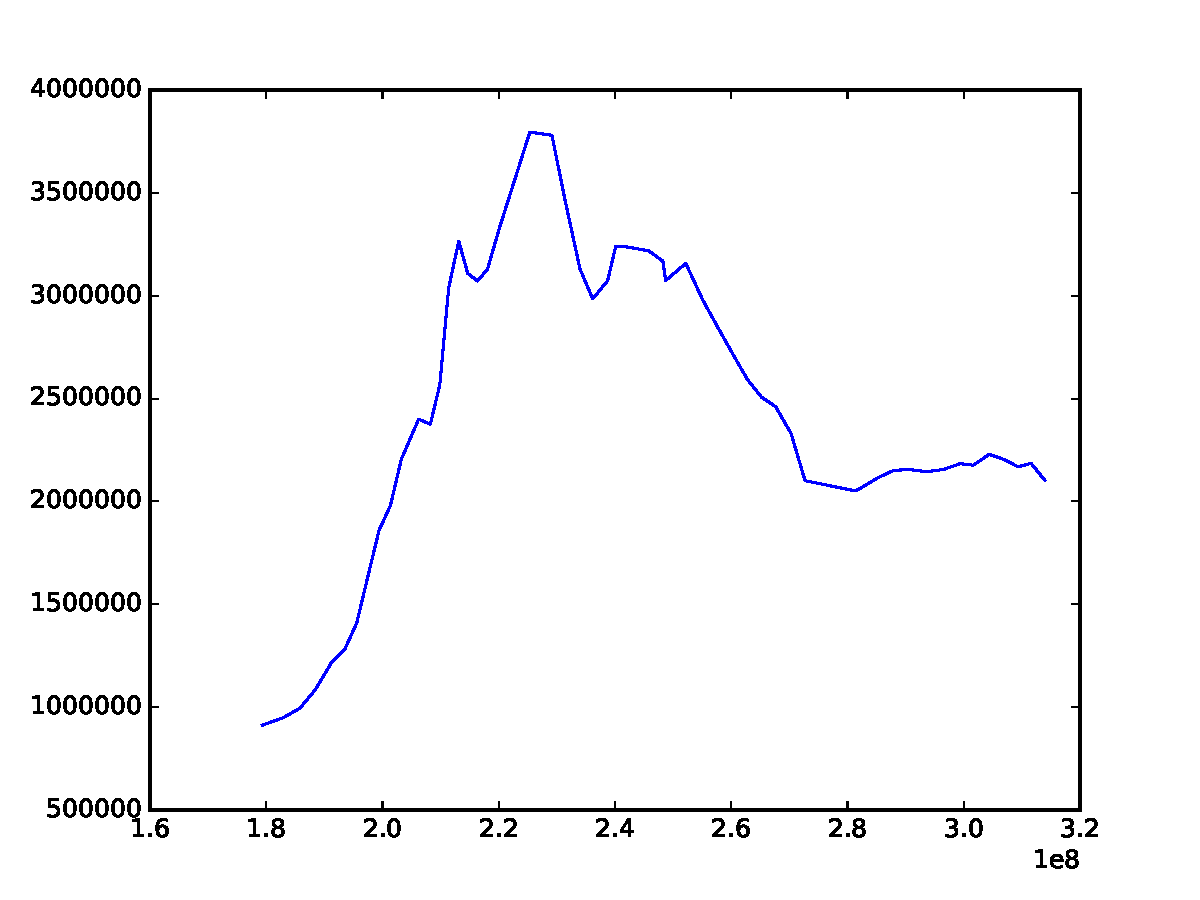
\includegraphics[width=\textwidth]{pltBurglary.pdf}
    \end{minipage}
    \quad
    \begin{minipage}[b]{0.48\textwidth}
    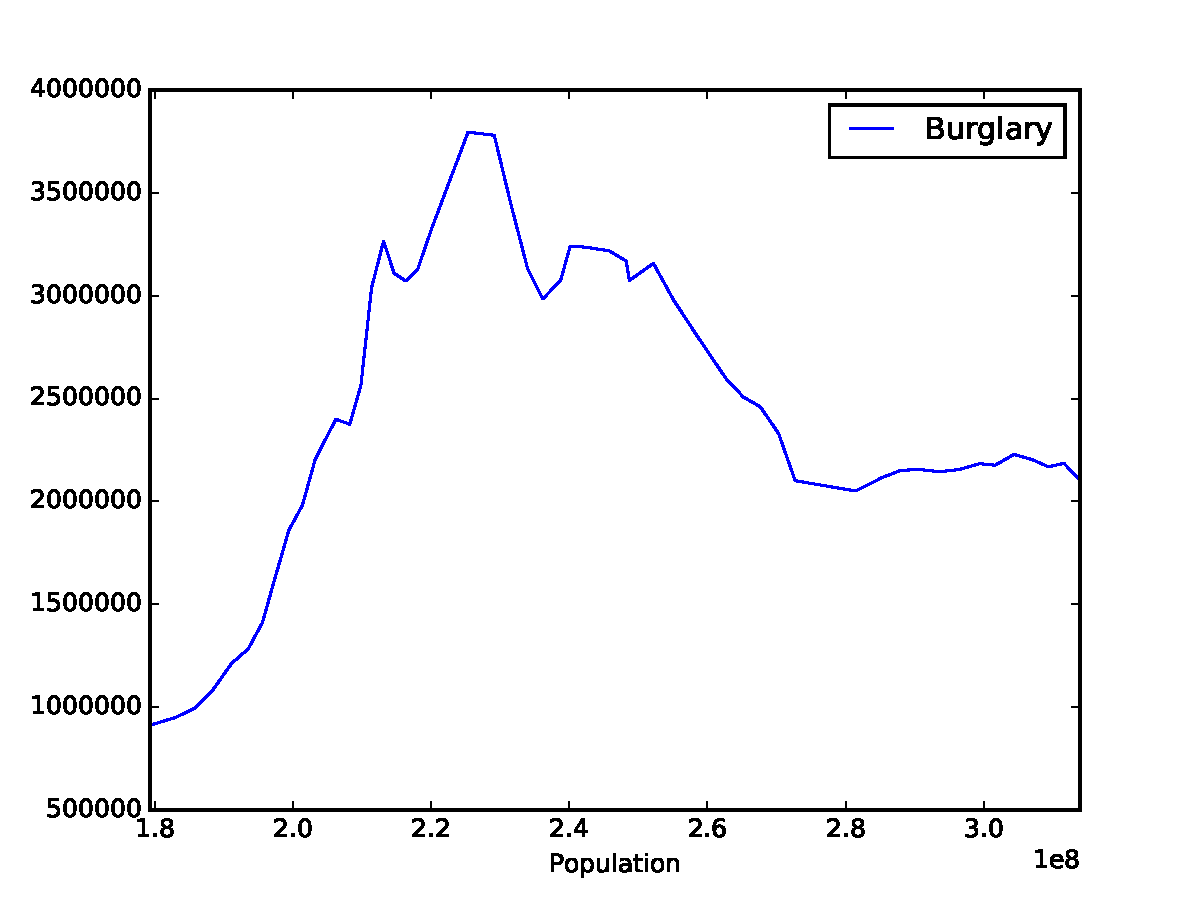
\includegraphics[width=\textwidth]{dfBurglary.pdf}
    \end{minipage}
    \caption{On the left, the result of \li{plt.plot()}. On the right, the result of \li{DataFrame.plot()}}
    \label{fig:intro2}
\end{figure}

Standard matplotlib keyword arguments can be passed in as usual to \li{DataFrame.plot()}.
This includes the ability to produce subplots quickly, modify the linestyle, and so on.

\begin{lstlisting}
>>> crime.plot(subplots=True, layout=(4,3), linewidth=3, style="--", legend=False)
>>> plt.show()
\end{lstlisting}

\subsection*{Bar Plots}

By default, the data frame's \li{plot()} function creates a line plot.
We can create other types of plots easily by specifying the keyword \li{kind}.
For example, bar plots are particularly useful for comparing several categories of data over time, or whenever there is a sense of progression in the index.
Bar plots tend to give a little more detail than line plots, though line plots are the better choice when there are many data points.
As an example, we compare three different types of crime over the last 5 years contained in the crime data set.
% Like histograms, bar plots can be stacked.

\begin{lstlisting}
# Each call to plot() makes a separate figure automatically.
>>> crime.iloc[-5:][["Aggravated-assault", "Violent", "Burglary"]].plot(kind="bar")
>>> crime.iloc[-5:][["Aggravated-assault", "Violent", "Burglary"]].plot(kind="bar", stacked=True, legend=False)
>>> plt.show()
\end{lstlisting}

\begin{figure}[H] % Bar Plots
    \centering
    \begin{minipage}[b]{.48\textwidth}
    	 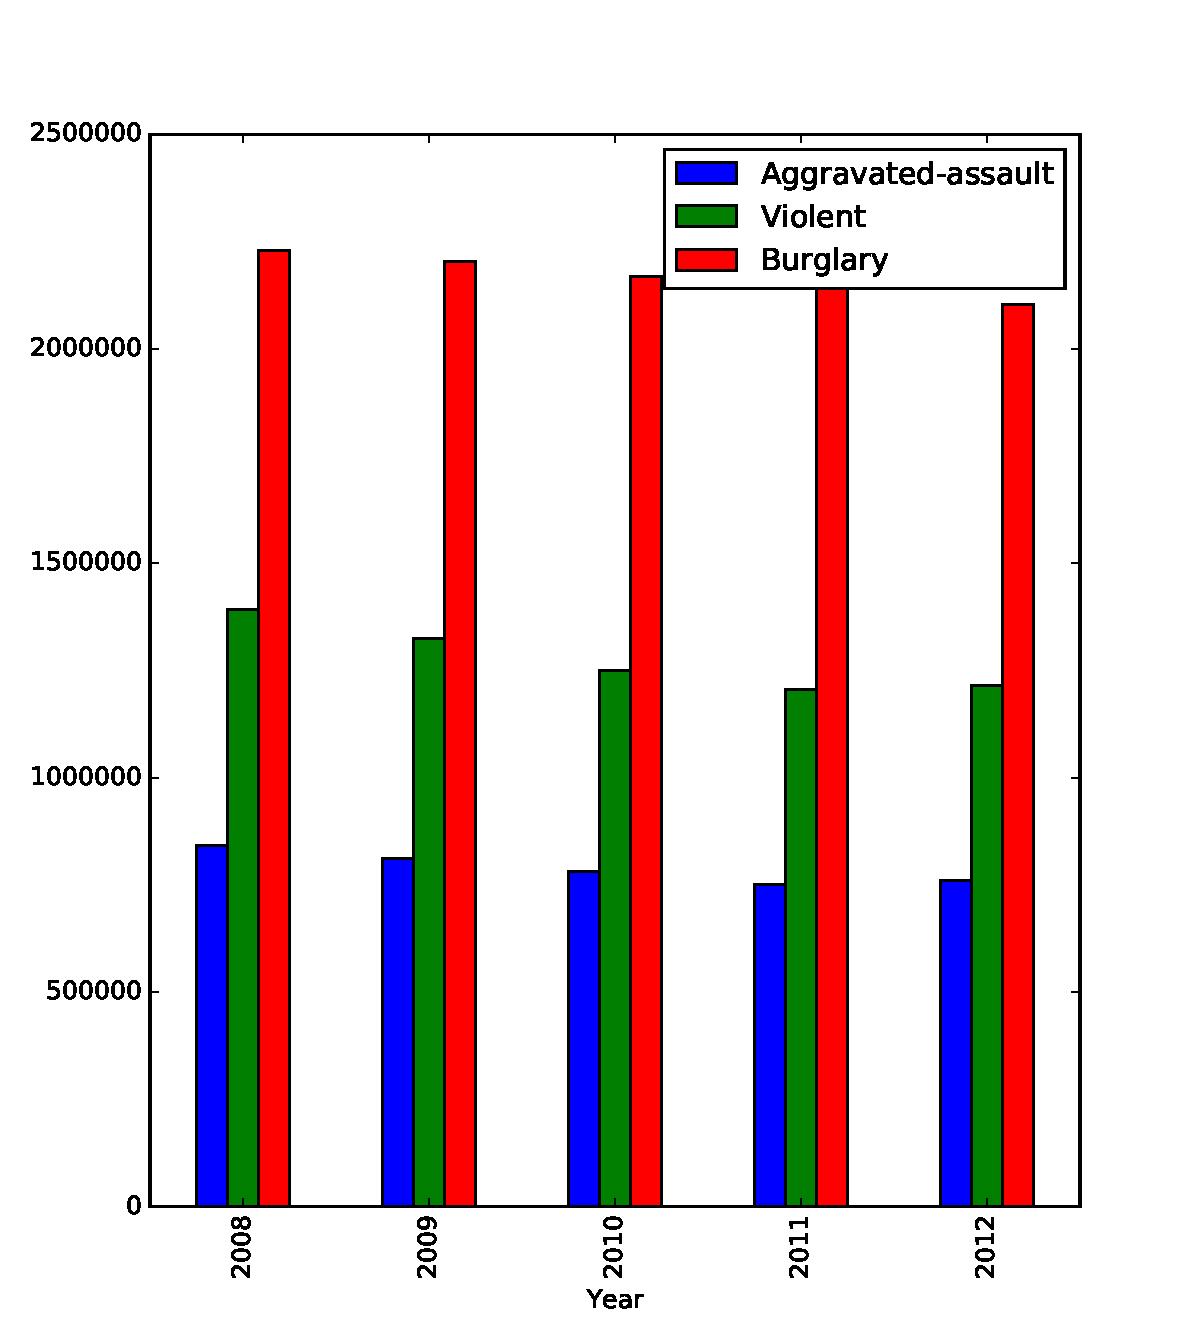
\includegraphics[width=\textwidth]{bar1.pdf}
	 \label{fig:overlap_hist}
    \end{minipage}
    \quad
    \begin{minipage}[b]{.48\textwidth}
    	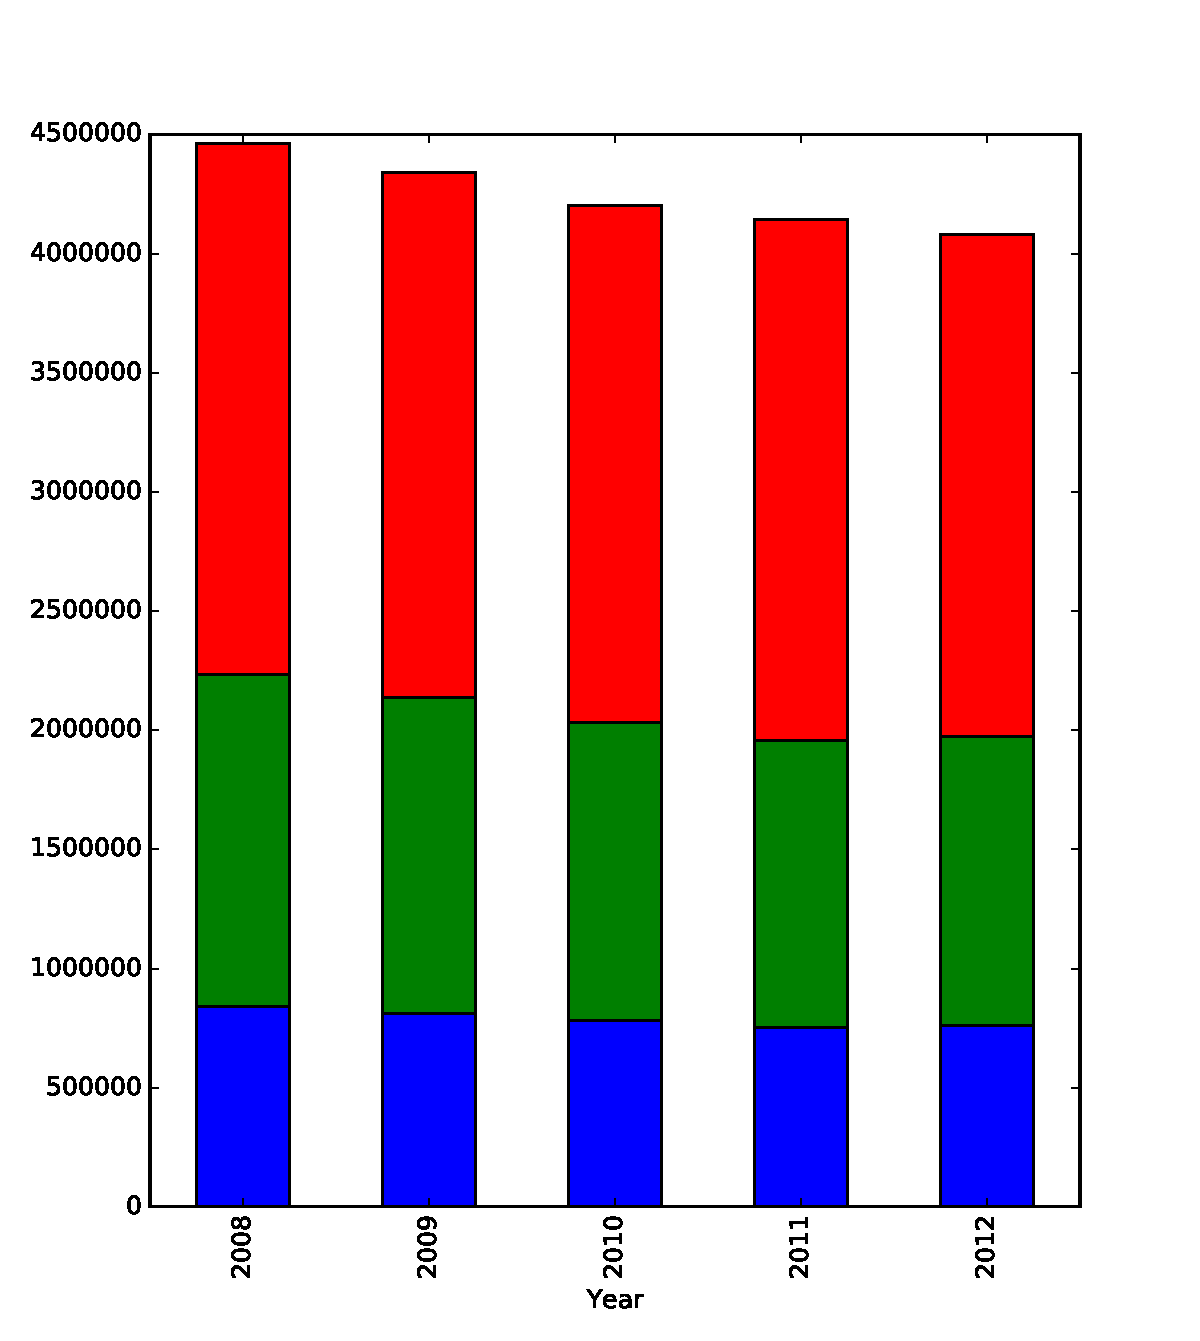
\includegraphics[width=\textwidth]{bar2.pdf}
	\label{fig:stacked_hist}
    \end{minipage}
\end{figure}

\subsection*{Problem \#1}
The \li{pydataset} module\footnote{Run \li{pip install pydataset} if needed} contains numerous data sets stored as Pandas data frames.
\begin{lstlisting}
from pydataset import data
# "data" is a Pandas data frame with IDs and descriptions.
# Call data() to see the entire list.
# To load a particular data set, enter its ID as an argument to data().
titanic_data = data("Titanic")
# To see the information about a data set, give data() the dataset_id with show_doc=True.
data("Titanic", show_doc=True)
\end{lstlisting}
Examine the data sets with the following \li{pydataset} IDs:
\begin{enumerate}
\item \li{nottem}: Average air temperatures at Nottingham Castle in Fahrenheit for 20 years.
\item \li{VADeaths}: Death rates per 1000 in Virginia in 1940.
\item \li{Arbuthnot}: Ratios of male to female births in London from 1629-171.
\end{enumerate}
Use line and bar plots to visualize each of these data sets.
Decide which type of plot is more appropriate for each data set, and which columns to plot together.
Write a short description of each data set based on the docstrings of the data and your visualizations.

\subsection*{Histograms}

Line and bar plots work well when there is a logical progression in the index, such as time.
However, when frequency of occurence is more important than the location of the data, histograms and box plots can be more informative.
Use \li{plot(kind="hist")} to produce a histogram.
Standard histogram options, such as the number of bins, are also accepted as keyword arguments.
The \li{alpha} keyword argument makes each bin slightly transparent.

\begin{lstlisting}
>>> crime[["Total", "Property"]].plot(kind="hist", alpha=.75)
>>> plt.show()
\end{lstlisting}

Alternatively, the bins can be stacked on top of each other by setting the \li{stacked} keyword argument to \li{True}.
We can also mke the histogram horizontal by seting the keyword  \li{orientation} to ``horizontal''.

\begin{lstlisting}
>>> crime[["Total", "Property"]].plot(kind="hist", stacked=True, orientation="horizontal")
>>> plt.show()
\end{lstlisting}

\begin{figure}[H] % Histograms
    \centering
    \begin{minipage}[b]{.48\textwidth}
    	 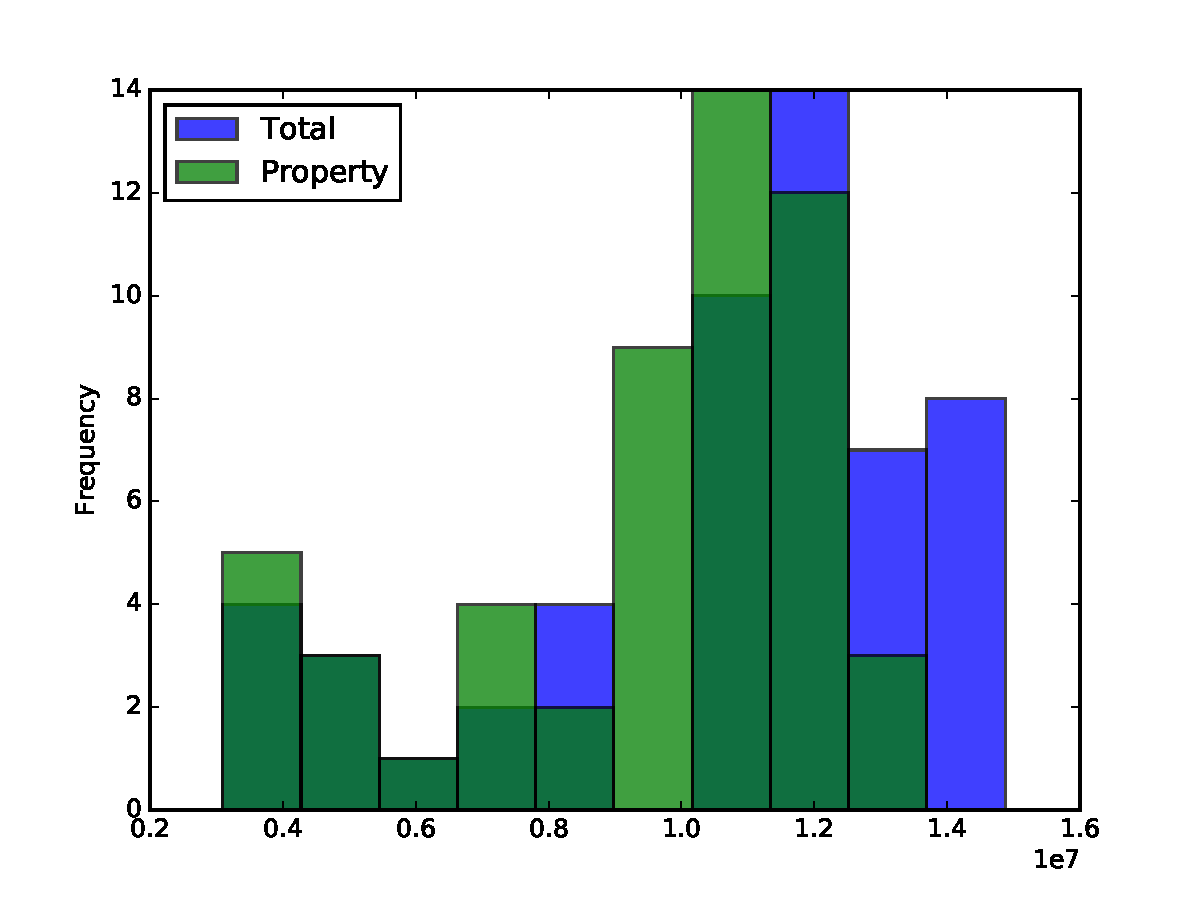
\includegraphics[width=\textwidth]{hist3.pdf}
	 \label{fig:overlap_hist}
    \end{minipage}
    \quad
    \begin{minipage}[b]{.48\textwidth}
    	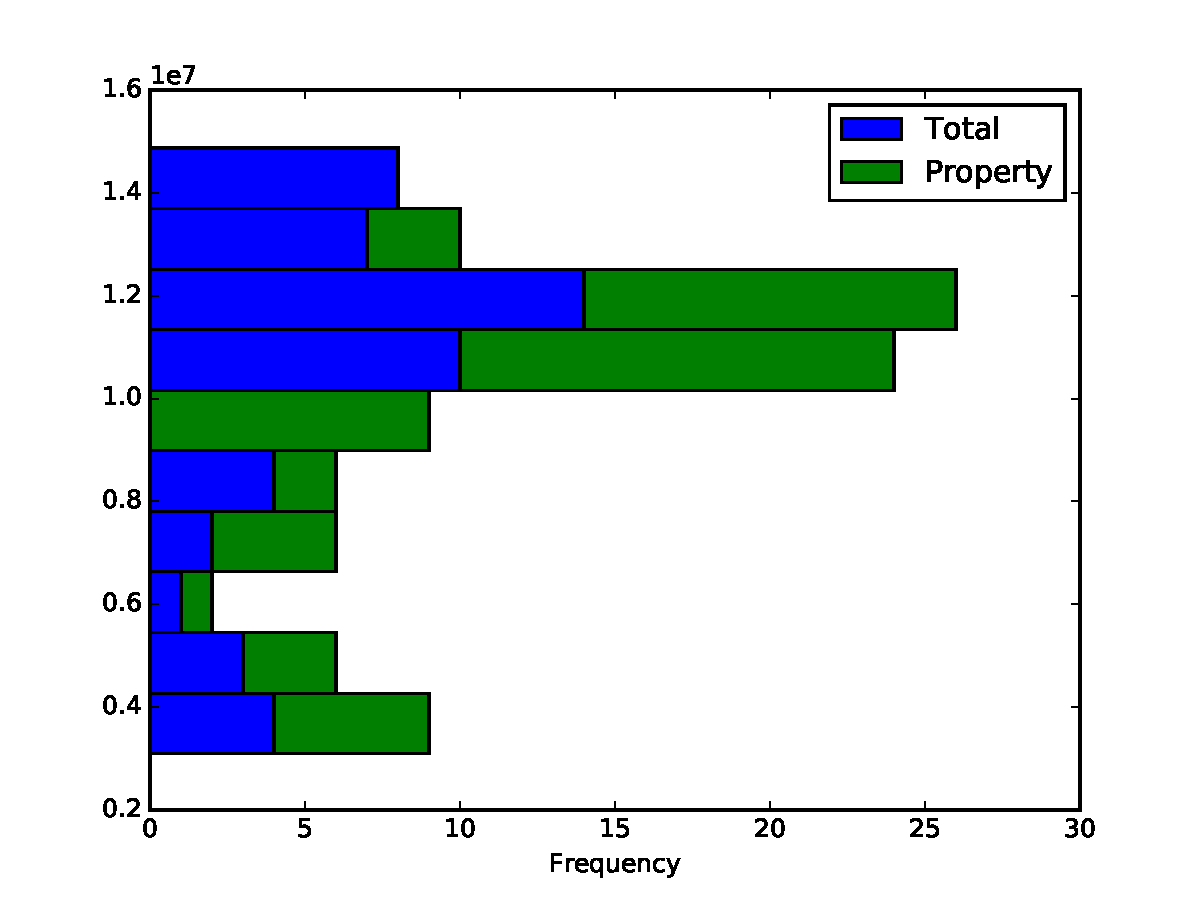
\includegraphics[width=\textwidth]{hist4.pdf}
	\label{fig:stacked_hist}
    \end{minipage}
\end{figure}

\subsection*{Box Plots}

Sometimes it is helpful to visualize a distribution of values using the box-and-whisker plot which is commonly taught in elementary school, which
displays the median, first and third quartiles, and outliers.
Like the previous examples, select the columns to examine and plot them with \li{plot()}.
To switch the orientation, use \li{vert=False}.

\begin{lstlisting}
crime[["Robbery", "Aggravated-assault", "Vehicle-Theft"]].plot(kind="box")
plt.show()
\end{lstlisting}

\begin{figure}[H] % Box Plots
    \centering
    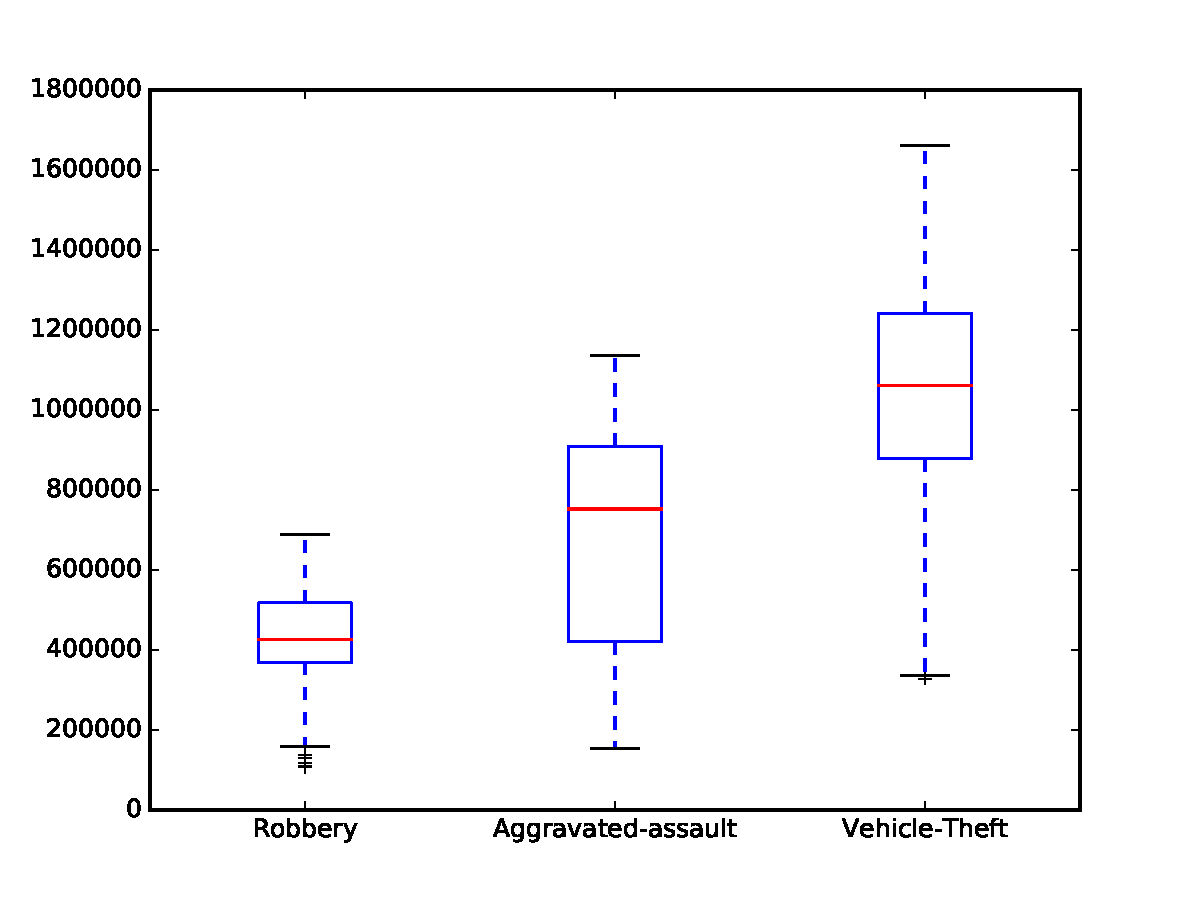
\includegraphics[width=.75\textwidth]{box1.pdf}
    \label{fig:box}
\end{figure}

\subsection*{Problem \#2}
Examine the data sets with the following \li{pydataset} IDs:
\begin{enumerate}
\item \li{trees}: Girth, height and volume for black cherry trees.
\item \li{road}: Road accident deaths in the United States.
\item \li{birthdeathrates}: Birth and death rates by country.
\end{enumerate}
Use histograms and box plots to visualize each of these data sets.
Decide which type of plot is more appropriate for each data set, and which columns to plot together.
Write a short description of each data set based on the docstrings of the data and your visualizations.


% NATHANIEL ===================================================================

\subsection*{Scatter Plots}
%Probably use the movie data here, compare with online images that are very similar to show the sophisication of the package.  I still think the movie data would be cool although they never got the cleaned up data to us.  Something similar wouldn't be too hard with the movie data

Scatter plots are one of the most commonly used type of plot and have a simple implementation in pandas. Unlike other plotting commands, \li{scatter} needs both an \li{x} and a \li{y} column as arguments.


\begin{lstlisting}
>>> mammal_speed = data("Mammals")
>>> mammal_speed.plot(kind="scatter", x="weight", y="speed"))
>>> plt.show()
\end{lstlisting}


The package includes many more scatter plot features which can be used to make the plots easier to understand.  For example, we can change the size of the point based on another column.  Consider the pydataset \li{HairEyeColor}, which contains the hair and eye color of various individuals. A scatter plot of hair color vs eye color is relatively useless unless we can see the frequencies with which each combination occurs.  Including the keyword argument \li{s} allows us to control the size of each point.  This can be set to a fixed value or the value in another column.  In the example below, the size of each point is set to the frequency with which each observation occurs.  

\begin{lstlisting}
>>> hec = data("HairEyeColor")
>>> X = np.unique(hec["Hair"], return_inverse=True)
>>> Y = np.unique(hec["Eye"], return_inverse=True
>>> hec["Hair"] = X[1]
>>> hec["Eye"] = Y[1]
>>> hec.plot(kind="scatter", x="Hair", y="Eye", s=hec["Freq"]*20)
>>> plt.xticks([0,1,2,3], X[0])
>>> plt.yticks([0,1,2,3], Y[0])
>>> plt.show()
\end{lstlisting}

\begin{figure}[H] 
    \centering
    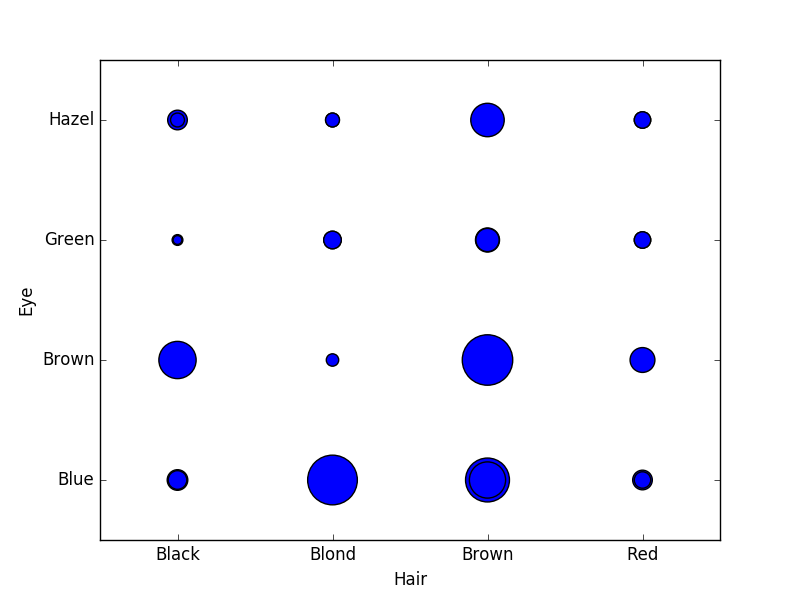
\includegraphics[width=.75\textwidth]{HairEyeColorscatter.png}
    \caption{Frequency of Hair-Eye Color Combinations}
\end{figure}


\subsection*{Hexbins}
While scatter plots are a great visualization tool, they can be uninformative for large datasets.  It is nearly impossible to tell what is going on in a large scatter plot, and the visualization is therefore of little value.  Hexbin plots solve this problem by plotting point density in hexagonal bins.  With hexbins, the structure of the data is easy to see despite the noise that is still present. 
Following is an example using pydataset's \li{sat.act} plotting the SAT Quantitative score vs ACT score of students


\begin{lstlisting}
>>> satact = data("sat.act")
>>> satact.plot(kind="scatter", x="ACT", y="SATQ")
>>> satact.plot(kind="Hexbin", x="ACT", y="SATQ", gridsize=20)
>>> plt.show()
\end{lstlisting}

Note the scatter plot in Figure 4. While we can see the structure of the data, it is not easy to differentiate the densities of the areas with many data points. Compare this now to the hexbin plot in Figure 5.  The two plots are clearly similar, but with the hexbin plot we have the added dimension of density.   
\begin{figure}[H] 
    \centering
    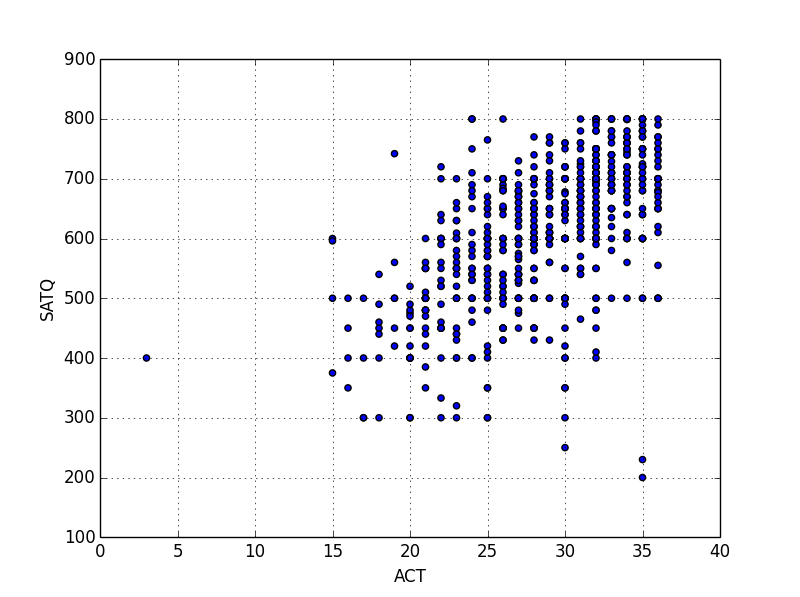
\includegraphics[width=.75\textwidth]{scatter.png}
    \caption{Scatter Plot}
\end{figure}

A key factor in creating an informative hexbin is choosing an appropriate \li{gridsize} parameter. This determines how large or small the bins will be. A large gridsize will give many small bins and a small gridsize gives a few large bins. Figure 6 shows the effect of changing the gridsize from 20 to 10.
\begin{figure}[H]
    \centering
    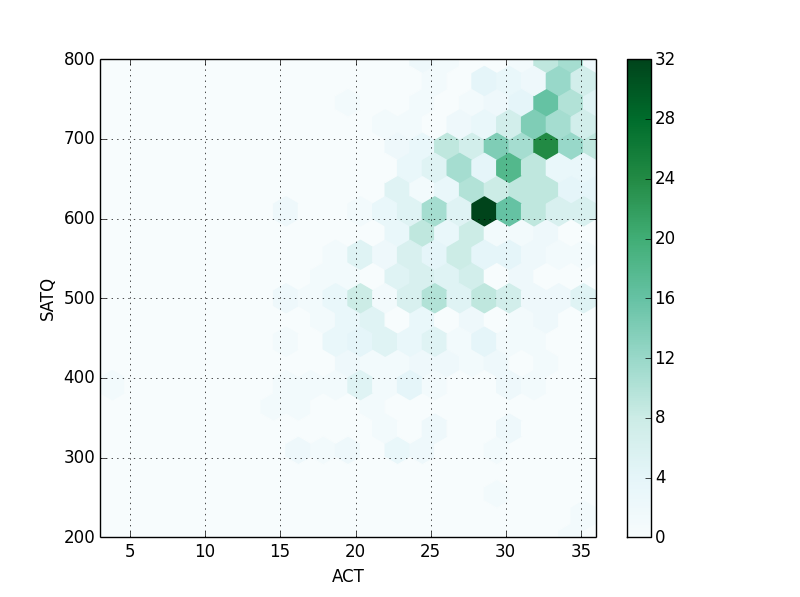
\includegraphics[width=.75\textwidth]{hexbin2.png}
    \caption{Hexbin Plot With Gridsize 20}
\end{figure}



\begin{figure}[H]
    \centering
    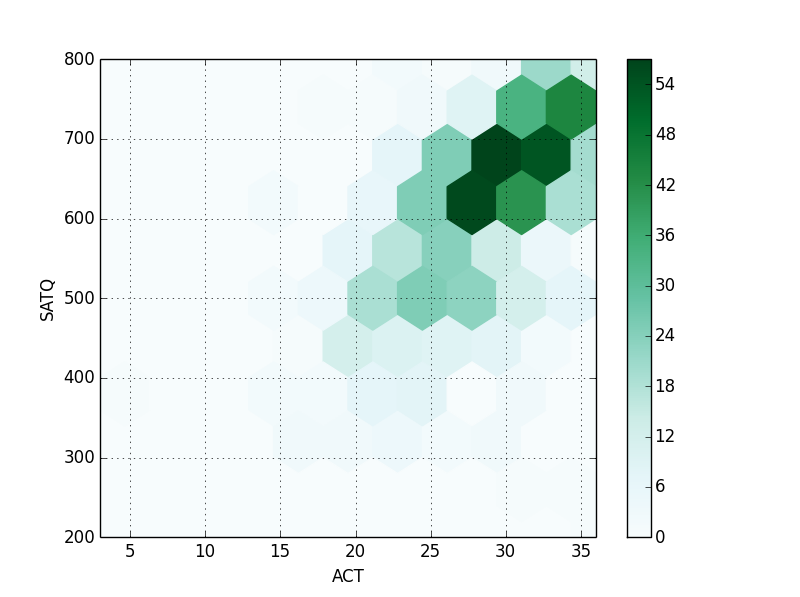
\includegraphics[width=.75\textwidth]{hexbin.png}
    \caption{Hexbin Plot With Gridsize 10}
\end{figure}





\subsection*{Lag Plot}
 We are frequently interested in whether or not data which we have collected is random. Lag plots are used to investigate the randomness of a dataset. If the data is in fact random, then the lag plot will exhibit no structure, while nonrandom data will exhibit some kind of structure. Unfortunately, this does not give us an idea of what exactly that structure may be, but it is a quick and effective way to investigate the randomness of a given dataset.
\begin{lstlisting}
>>> from pandas.tools.plotting import lag_plot
>>> randomdata = pd.Series(np.random.rand(1000))
>>> lag_plot(randomdata)
>>> plt.show()

>>> structureddata = pd.Series(np.sin(-np.pi, np.pi, num=1000))
>>> lag_plot(structureddata)
>>> plt.show()
\end{lstlisting}


\begin{figure}[H]
    \centering
    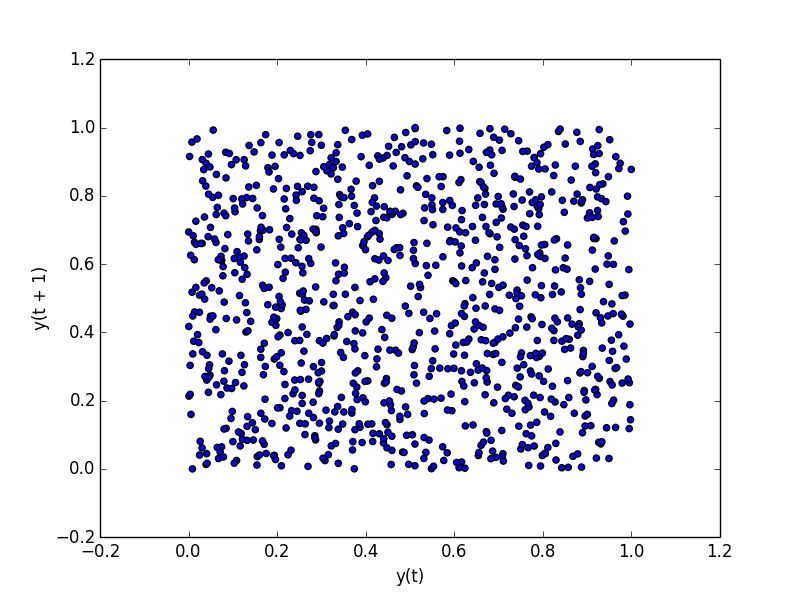
\includegraphics[width=.75\textwidth]{randomdata.png}
    \caption{Lag Plot of Random Data}
\end{figure}


\begin{figure}[H]
    \centering
    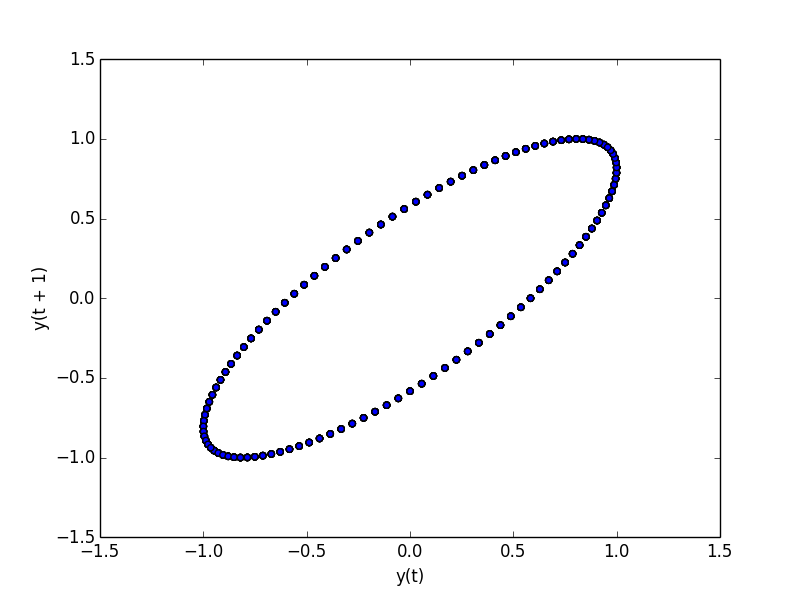
\includegraphics[width=.75\textwidth]{structureddata.png}
    \caption{Lag Plot of Sine Wave}
\end{figure}

\subsubsection*{Problem \#3} Choose a dataset provided in the \li{pydataset} and produce scatter and hexbin plots demonstrating some characteristic of the data. A list of datasets in the \li{pydataset} module can be produced using the \li{data()} command.


For more types of plots available in Pandas and further examples, see \url{http://pandas.pydata.org/pandas-docs/stable/visualization.html}.

% AMELIA =====================================================================
\section*{Data Visualization}

Visualization is much more than a set of pretty pictures scattered throughout a paper for the sole purpose of providing candy-colored filler.
When properly implemented, data visualization is a powerful tool for analysis and communication. 
In this section we discuss the process of making deliberate, effective, and efficient design decisions.

\subsection*{Catching all of the Details}

Consider the figure entitled ``Plot 1''. 
What does it depict?
We can tell from a simple glance that it is a scatter plot of positively correlated data of some kind, with \li{temp}--likely temperature--on the $x$ axis and \li{cons} on the $y$ axis. 
However, the picture is not really communicating anything about the dataset. We have not specified the units for the $x$ or the $y$ axis, we have no idea what \li{cons} is, and we don't even know where the data came from in the first place. 

\begin{figure}[H] 
    \centering
    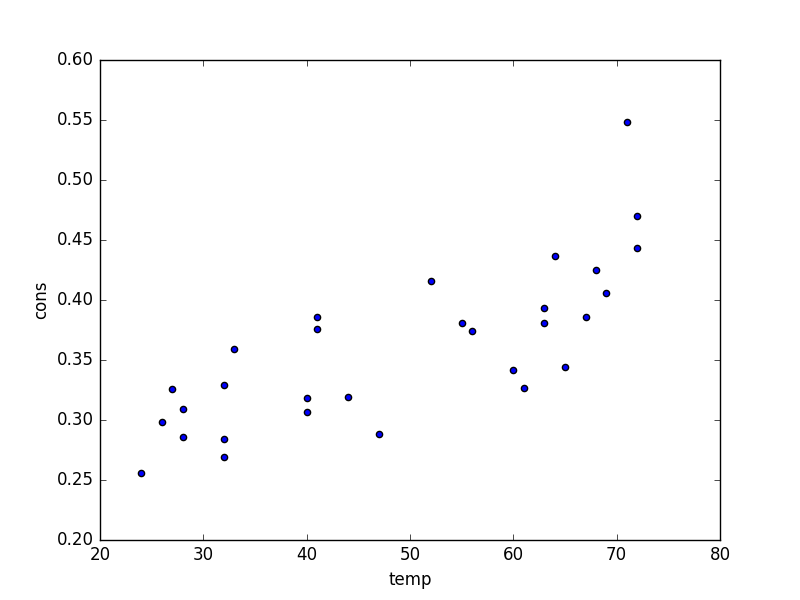
\includegraphics[width=.75\textwidth]{Nolabels.png}
    \caption{Plot 1}
    \label{fig:aplot}
\end{figure}

\subsubsection*{Labels, Legends, and Titles}
In a homework or lab setting, we sometimes (mistakenly) think that it is acceptable to leave off appropriate labels, legends, titles, and sourcing.
In a published report or presentation, this kind of carelessness is confusing at best and (when the source is not included) plagiaristic at worst.
Here, we offer a brief overview of the pandas code that will allow us to add these vital elements.

Consider again ``Plot 1''. 
This figure comes from the \li{Icecream} dataset within the \li{pydataset} package, which we store here in a dataframe and then plot:
\begin{lstlisting}
>>> icecream = data("Icecream")
>>> icecream.plot(kind="scatter", x="temp", y="cons")
\end{lstlisting}

We have at this point reproduced the rather substandard plot in Figure 9.
Using \li{data('Icecream', show\_doc=True)} we find the following information:
\begin{enumerate}
    \item The dataset details ice cream consumption via four-weekly observations from March 1951 to July 1953 in the United States.
    \item \li{cons} corresponds to ``consumption of ice cream per head'' and is measured in pints.
    \item \li{temp} corresponds to temperature, degrees Fahrenheit.
    \item The listed source is: ``Hildreth, C. and J. Lu (1960) \_Demand relations with autocorrelated disturbances\_, Technical Bulletin No 2765, Michigan State University.''
\end{enumerate}

We add these important details using the following code.
As we have seen in previous examples, Pandas automatically generates legends when appropriate.
However, although Pandas also automatically labels the $x$ and $y$ axes, our data frame column titles may be insufficient.
Appropriate titles for the $x$ and $y$ axes must also list appropriate units. 
For example, the $y$ axis should specify that the consumption is \emph{per head} with unit \emph{pints}, in place of the ambigious label \li{cons}.
\begin{lstlisting}
>>> icecream = data("Icecream")
# Set title via the title keyword argument
>>> icecream.plot(kind="scatter", x="temp", y="cons", title="Ice Cream Consumption in the U.S., 1951-1953",)
# Override pandas automatic labelling using xlabel and ylabel
>>> plt.xlabel("Temp (Farenheit)")
>>> plt.ylabel("Consumption per head (pints)")
>>> plt.show()
\end{lstlisting}

Unfortunately, there is no explicit function call that allows us to add our source information.
To arbitrarily add the necessary text to the figure, we may use either \li{plt.annotate} or \li{plt.text}. 
\begin{lstlisting}
>>> plt.text(20, .1, "Source: Hildreth, C. and J. Lu (1960) _Demand relations with autocorrelated disturbances_\nTechnical Bulletin No 2765, Michigan State University.", fontsize=7)
\end{lstlisting}
Both of these methods are imperfect, however, and can normally be just as easily replaced by a caption attached to the figure in your presentation or document setting. 
We again reiterate how important it is that you source any data you use. Failing to do so is plagiarism.

Finally, we have a clear and demonstrative graphic:

\begin{figure}[H] 
    \centering
    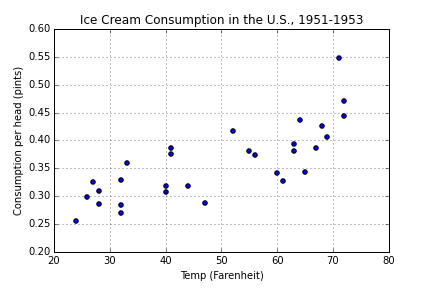
\includegraphics[width=.75\textwidth]{Icecream.png}
    \caption{Source:  Hildreth, C. and J. Lu (1960) \_Demand relations with autocorrelated disturbances\_, Technical Bulletin No 2765, Michigan State University.}
    \label{fig:aplot}
\end{figure}

\subsubsection*{Problem \#4}
Return to the plots you generated in problem one (datasets \li{nottem}, \li{VADeaths}, and \li{Arbuthnot}).
Reproduce and modify these plots to include:
\begin{itemize}
\item A clear title, with relevant information for the period or region the data was collected in.
\item Axes that specify units.
\item A legend (for comparison data).
\item The source. You may include the source information in your plot or print it after the plot at your discretion.
\end{itemize}
Note that in this and all subsequent problems, points will be taken off if any of these items are partially or fully missing from your graphs.


\begin{comment}
\subsubsection*{Colors and Scaling}
This discussion will draw heavily from discussions on visualization from recent conferences such as SciPy and Vis.
A lot of research and effort has been put into color choice.
We will also briefly discuss choosing an appropriate scale for the graph.
\end{comment}


\subsection*{Choosing the Right Plot}
Now that we know how to add the appropriate details for remaining plots, we return to the fundamental question of data visualization--which plot is the right plot for your data? 
In previous sections, we have already discussed the various strengths and weaknesses of available pandas plotting techniques.
At this point, we know how to visualize data using bar charts and histograms or scatter plots and hexbins. 
However, perfectly plot-ready data sets--organized by a simple continuum or a convenient discrete set--are few and far between.
In the real world, it is rare to find a dataframe that is already ready to become a meaningful visual.

As such, deciding how to organize and group the data within your dataframe is one of the most important parts of ``choosing the right plot''.

\begin{comment}
Discuss the importance of choosing the right plot for your data, and analyzing what you want to communicate.
This section will probably use 1-3 datasets from PyDataset describing diseases.
Since these datasets are easy to download and use, that will be a good way to compare how different datasets match certain plots better, and then similarly divide certain aspects of the data into different plots.

One example here will be the PyDataset's AIDS dataset.
In addition to its categories of infection and induction periods, we can compare adult cases to children using a bar chart, or simply focus on one of these two using a scatter plot.
There are many different ways to describe the data, here we will discuss how what we want to display effects the plot we choose.
\end{comment}

\subsubsection*{Groupby}
Many datasets are simply composed of tables of individuals, with a list of classifiers associated with each one.
Data like this is difficult to sensibly plot in its raw format.

For example, consider the \li{msleep} dataset (found in \li{pydataset}). 
Each row consists of a single type of mammal and its corresponding identifiers, including genus and order, as well as sleep measurements such as total amount of sleep (in hours) and REM sleep, in hours.
When we try to plot this data using plt.plot, the individual data points do not demonstrate overall trends.
\begin{lstlisting}
>>> msleep = data("msleep")
>>> msleep.plot(y="sleep_total", title="Mammalian Sleep Data", legend=False)
>>> plt.xlabel("Animal Index")
>>> plt.ylabel("Sleep in Hours")
>>> plt.show()
\end{lstlisting}
The above code results in Figure 11.
\begin{figure}[H] 
    \centering
    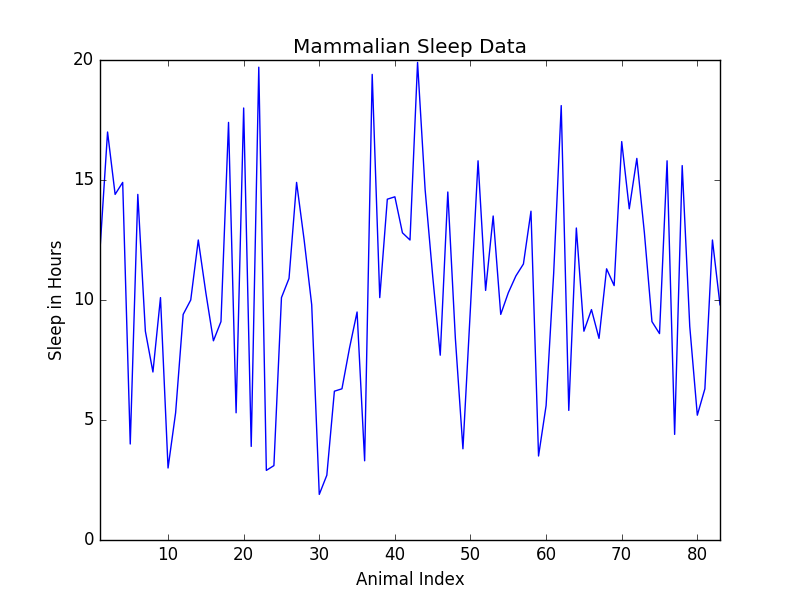
\includegraphics[width=.75\textwidth]{Msleep1.png}
    \caption{Source:  Proceedings of the National Academy of Sciences, 104 (3):1051-1056, 2007. Updates from V. M. Savage and G. B. West, with additional variables supplemented by Wikipedia.}
    \label{fig:aplot}
\end{figure}
This seemingly random set of connected data points is not particularly revealing.

We thus decide to approach our dataset using pandas' powerful \li{groupby} method. 
Let's say that, for the \li{msleep} dataset, we want to visualize the differences in sleep data between herbivores, omnivores, insectivores and carnivores.
Then, we simply call the groupby method on the \li{vore} column to obtain a groupby object organized diet classification.
\begin{lstlisting}
>>> msleep = data("msleep")
>>> vore = msleep.groupby("vore")
\end{lstlisting}
You can also group the data by multiple columns, for example, both the \li{vore} and \li{order} classifications.
To group and view this data, simply use:
\begin{lstlisting}
>>> vorder = msleep.groupby(["vore", "order"])

# View groups within vorder
>>> vorder.describe
\end{lstlisting}

Pandas \li{groupby} objects are not lists of new dataframes associated with groupings.
They are better thought of as a dictionary or generator-like object which can be \emph{used} to produce the necessary groups.
However, if you want to work within a dataframe for a specific group, you may use the \li{get\_group()} method as follows:

\begin{lstlisting}
# Get carnivore group
>>> Carni = vore.get_group("carni")
# Get herbivore group
>>> Herbi = vore.get_group("herbi")
\end{lstlisting}

The \li{groupby} object includes many useful methods that can help us make visual comparisons between groups. 
The \li{mean()} method, for example, returns a new dataframe consisting of the mean values attached to each group.
For example, using this method on our \li{vore} object returns a nicely organized dataframe of the average sleep data for each mammalian diet pattern.
We can similarly create a dataframe of the standard deviations for each group.

At this point, we have a nicely organized dataset that can easily be turned into a bar chart.
Here, we use the \li{dataframe.loc} method to access three specific columns in the bar chart (\li{sleep_total}, \li{sleep_rem}, and \li{sleep_cycle}).
\begin{lstlisting}
>>> means = vore.mean()
>>> errors = vore.std()

>>> means.loc[:,["sleep_total", "sleep_rem", "sleep_cycle"]].plot(kind="bar", yerr=errors, title="Mean Mammallian Sleep Data")
>>> plt.xlabel("Mammal diet classification (vore)")
>>> plt.ylabel("Hours")
>>> plt.show()
\end{lstlisting}

\begin{figure}[H] 
    \centering
    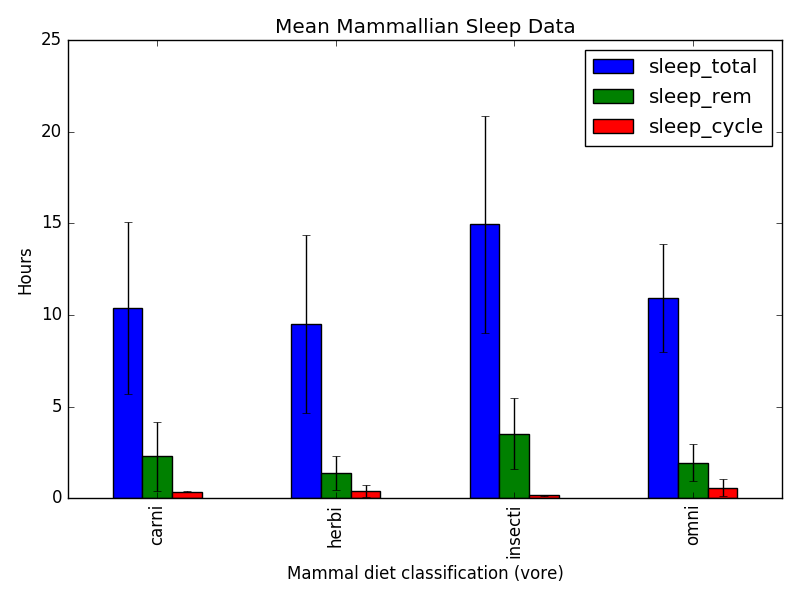
\includegraphics[width=.75\textwidth]{MeanMammal.png}
    \caption{Source:  Proceedings of the National Academy of Sciences, 104 (3):1051-1056, 2007. Updates from V. M. Savage and G. B. West, with additional variables supplemented by Wikipedia.}
    \label{fig:aplot}
\end{figure}

The pandas \li{groupby} object has many different methods.
We have discussed a few of these here; for more information please see: 
\begin{itemize}
    \item \url{http://pandas.pydata.org/pandas-docs/stable/generated/pandas.DataFrame.groupby.html}
    \item \url{http://pandas.pydata.org/pandas-docs/stable/groupby.html}
\end{itemize}
% Potential data sets: population density

% What to do about missing information (nans, zeros, etc).

% Probably a data set using disease
\subsubsection*{Problem \#5} 
Examine the \li{diamonds} dataset found in the \li{pydataset} module. 
This dataset contains the identifiers and attributes of 53,940  individual round cut diamonds. 
Using the \li{groupby} method, create three different visuals highlighting and comparing different aspects of the data.
This can be in the form of a single plot or comparative subplots.

Print a few sentences for each plot explaining what type of graph you used, why, and what we learn about the dataset from your plot.
Don't forget that points will be taken off for each plot without a title, clear labels, and sourcing. 

The following is an example of the kind of plot we are looking for. 
This example may not be used as one of your three plots.
\begin{figure}[H] % Matplotlib vs. Pandas
    \centering
    \begin{minipage}[b]{0.48\textwidth}
    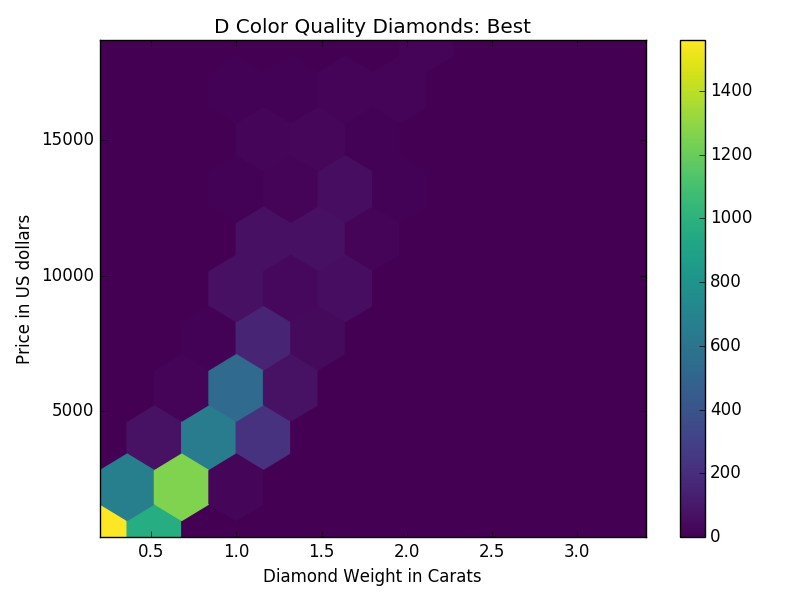
\includegraphics[width=\textwidth]{DiamondD.png}
    \end{minipage}
    \quad
    \begin{minipage}[b]{0.48\textwidth}
    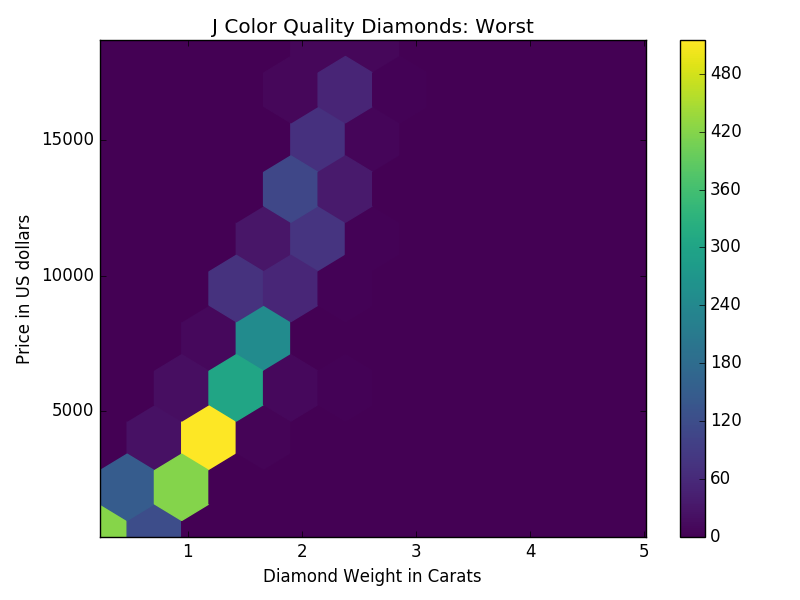
\includegraphics[width=\textwidth]{DiamondJ.png}
    \end{minipage}
    \caption{Source: Adopted from R Documentation}
    \label{fig:intro2}
\end{figure}

The code for the above figure is included here:
\begin{lstlisting}
>>> Diamonds = data("diamonds")
>>> DiaColor = Diamonds.groupby("color")
>>> Ddiamond = DiaColor.get_group("D")
>>> Jdiamond = DiaColor.get_group("J")

>>> Ddiamond.plot(kind="hexbin", x="carat", y="price", gridsize=10, title="D Color Quality Diamonds: Best", cmap="viridis")
>>> plt.ylabel("Price in US Dollars")
>>> plt.xlabel("Diamond Weight in Carats")
>>> plt.tight_layout()
>>> plt.show()

>>> Jdiamond.plot(kind="hexbin", x="carat", y="price", gridsize=10, title="J Color Quality Diamonds: Worst", cmap="viridis")
>>> plt.ylabel("Price in US Dollars")
>>> plt.xlabel("Diamond Weight in Carats")
>>> plt.tight_layout()
>>> plt.show()
\end{lstlisting}

We now analyze the plots.

The above plots were created using \li{groupby} on the diamond colors and then using a hexbin comparing carats to price for the highest and lowest quality diamonds, respectively. 
This hexbin is particularly revealing for each set of thousands of diamonds because it meaningfully displays concentration of datapoints. 
Matplotlib's new \li{viridis} colorplot, with a dark background, reveals bins that would have been invisible with a white background.
By comparing these plots, we note that the greatest number of J quality diamonds in the dataset are about 1.25 carats and \$4000 dollars in price, whereas the highest concentration of D quality diamonds are smaller and therefore cheaper. 
We may attribute this to D quality diamonds being rarer, but the colorbar on the side reveals that D diamond numbers are, in fact, far higher than those of the J color. 
Instead it is simply more likely that D quality diamonds of larger sizes are rarer than those of smaller sizes. 
Both hexbins reveal a linearity between diamond weight and diamond price, with D diamonds showing more variability and J diamonds displaying a strict linearity.

\end{document}
